\documentclass[../Main/Knit.tex]{subfiles}
\newpage

\subsection{Lab Worflow}
\label{chap:isoseq_labpipeline}
This section specficially describes the lab workflow for the library preparation for PacBio Iso-Seq. All details relating to sample preparation, cDNA synthesis and amplification can be found in \cref{ch:general_methods}.

The Iso-Seq lab protocol, as outlined in \cref{fig:isoseq_wholelab_protocol}, involved three main steps by i) converting total RNA transcripts to full-length cDNA using the Clontech SMARTer PCR cDNA synthesis kit, ii) amplification and purification of double-stranded cDNA, and iii) performing library preparation for long-read sequencing which involved constructing the SMRT bell library. Size selection was not performed with full-length transcript detection of up to 4 kB. For targeted transcriptome profiling with enrichment of target genes, all the steps in the workflow were the same with an additional step of target capture post ds-DNA amplification and pre-SMRT bell library, and usage of barcodes to allow multiplexing (\cref{fig:isoseq_targetedlab_protocol}). 

\begingroup
\parindent=0em
\etocsettocstyle{\rule{\linewidth}{\tocrulewidth}\vskip0.5\baselineskip}{\rule{\linewidth}{\tocrulewidth}}
\etocsetnexttocdepth{5}
\localtableofcontents 
\endgroup

\begin{figure}[htp]
	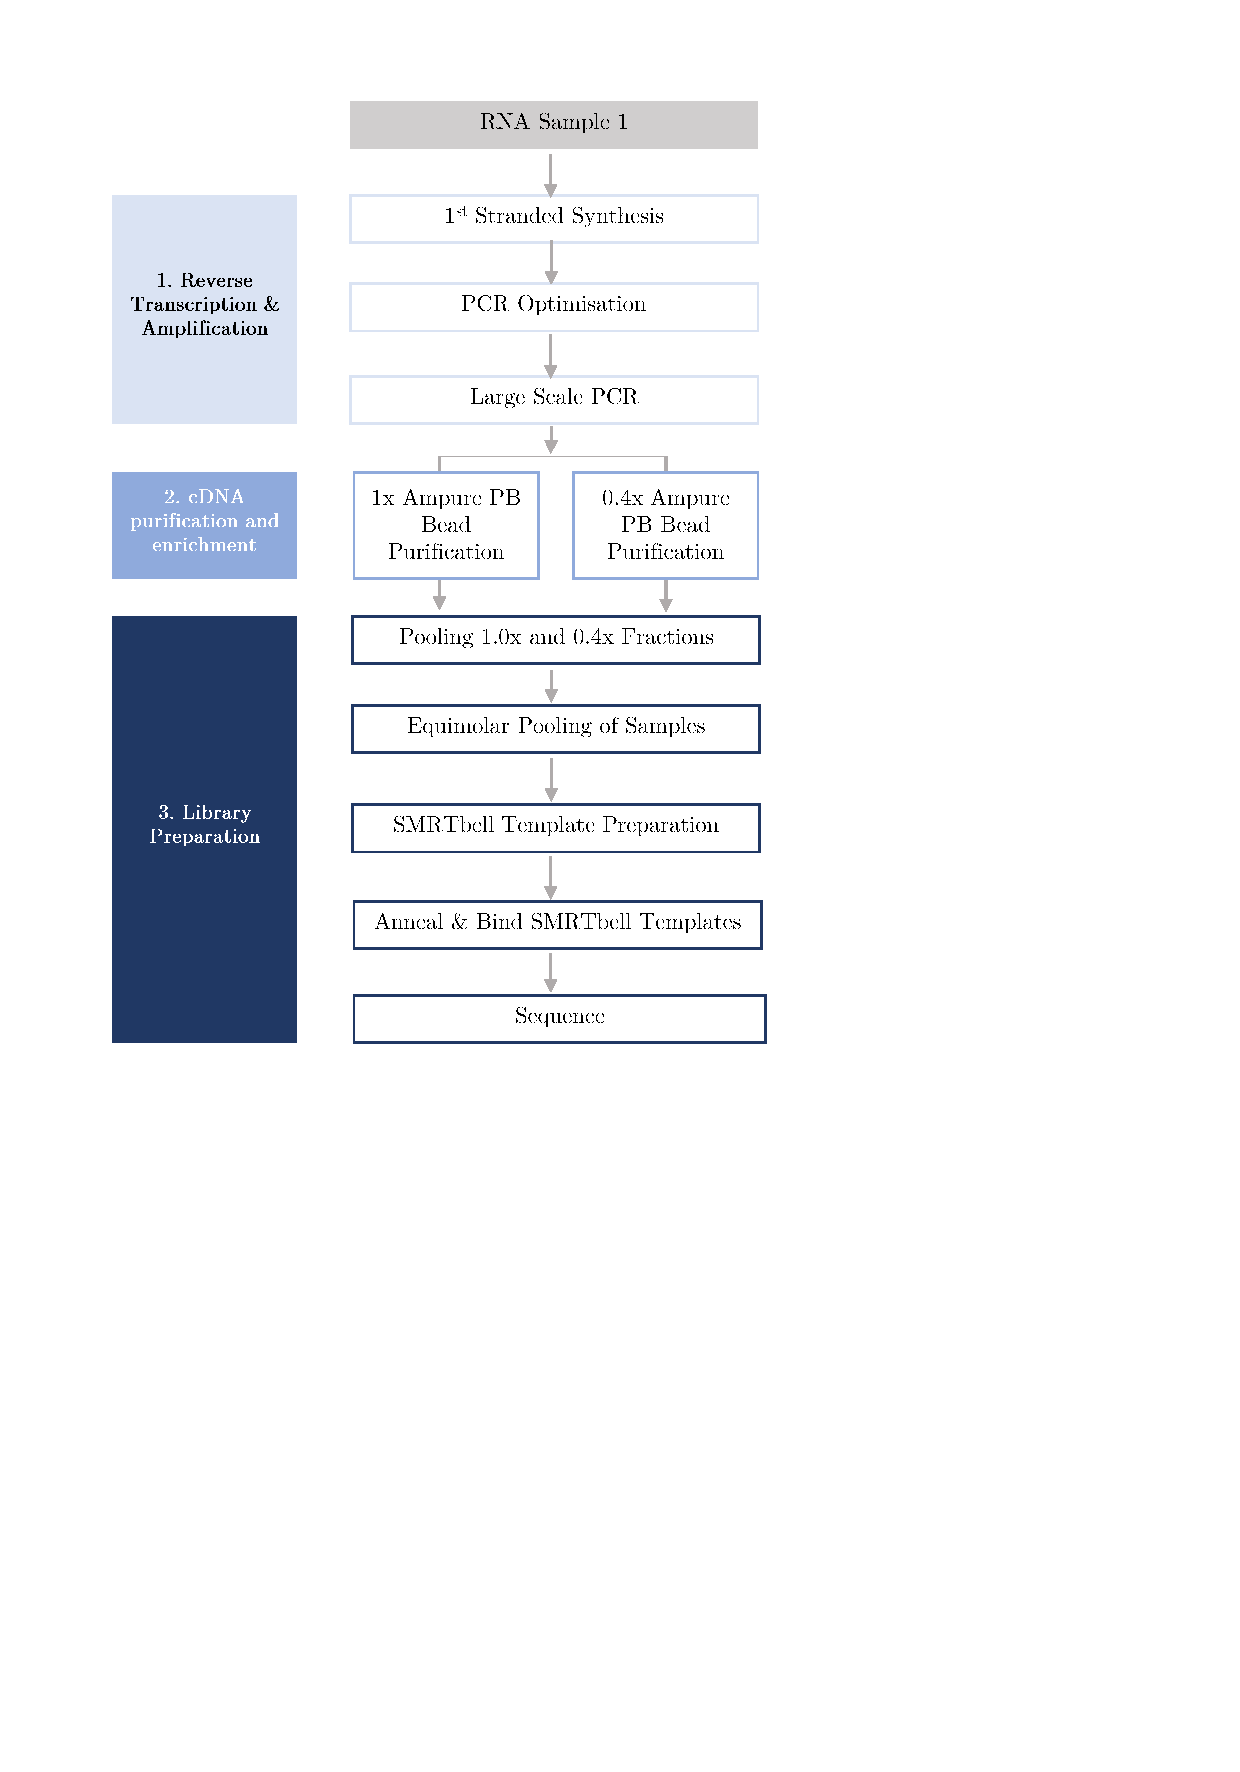
\includegraphics[page=1,trim={0 18cm 5cm 1cm},clip,scale = 0.6]{ProjectDevelopment_Figures}
	\captionsetup{width=0.95\textwidth}
	\caption[Iso-Seq Lab workflow used for whole transcriptome sequencing]%
	{\textbf{An overview of the lab Iso-Seq workflow used for whole transcriptome profiling}. The lab workflow, as adapted from official Iso-Seq protocol, involves three main steps: 1) reverse transcription and amplification of cDNA ( \cref{section:ch2_cDNA_synthesis_explanation}), 2) cDNA purification with ampure beads ( \cref{section:ch2_AMPure_explanation}) and 3) library preparation involving ligation of SMRT bell templates, and primer and polymerase binding (\cref{section:ch2_smrtbelltemplate_explanation})}
	\label{fig:isoseq_wholelab_protocol}
\end{figure}

\begin{figure}[]
	\begin{center}
		\includegraphics[page=2,trim={1cm 18cm 1cm 3cm},clip,scale = 0.45]{ProjectDevelopment_Figures}
	\end{center}
	\captionsetup{width=0.95\textwidth}
	\caption[Iso-Seq Lab workflow used for targeted transcriptome sequencing]%
	{\textbf{An overview of the lab Iso-Seq pipeline used for targeted transcriptome profiling}. The lab workflow for targeted transcriptome profiling involves all the steps in the standard Iso-Seq lab workflow (Figure \ref{fig:isoseq_wholelab_protocol}), with the addition of the target capture step (Boxed orange, Section \ref{section:ch2_targetcapture_explanation}) and the use of barcoded primers in reverse transcription (Boxed green and denoted here as Barcode 1 and Barcode n) to allow sample multiplexing (denoted here as Sample n, PacBio recommends 6-8 multiplexed samples per run). The list of barcodes can be found in \cref{tab:barcode_primers}}
	\label{fig:isoseq_targetedlab_protocol}
\end{figure}


\subsubsection{PCR optimisation and DNA Amplification}
After cDNA synthesis (described in \cref{section:ch2_cDNA_synthesis_explanation}), cDNA products were amplified using PCR (described in \cref{section:ch2_PCR_explanation}) to ensure sufficient material for sequencing. To minimise PCR bias (under or over-amplification), which can result in under or over representation of the different cDNA library size, the optimal number of PCR cycles for amplification with PrimeSTAR GXL DNA Polymerase (Clontech) was determined (\cref{fig:pcr_optimisation_gel_eg}). This was achieved by collecting 5uL PCR aliquots every two cycles (cycle 10, 12, 14, 16, 18, 20) followed by visualisation of cDNA products on a 1.5\% Agarose gel electrophoresis with ethidium bromide. Large scale PCR amplification was then subsequently performed using the optimal number of cycles.

%Single-stranded DNA generated from SMARTer PCR synthesis kit in the official Iso-Seq protocol was amplified by PCR using PrimeSTAR GXL DNA Polymerase (ClonTech). Also performed for targeted sequencing. 

\begin{figure}[htp]
	\begin{center}
		\includegraphics[page=3,trim={1cm 24cm 10cm 1cm},clip,scale = 0.9]{ProjectDevelopment_Figures.pdf}
	\end{center}
	\captionsetup{width=0.95\textwidth}
	\caption[Example of Agarose gel to determine optimum number of PCR cycles for amplification]%
	{\textbf{PCR optimisation is required to determine optimum number of cycles}. Shown is an agarose gel of Human Brain Total RNA after 1st strand cDNA synthesis and PCR amplification through cycles 8 to 18, with PCR aliquots collected during respective cycles. In this example, 10 cycles were determined to be the optimum number for large-scale amplification. While smear distribution from 8 and 10 cycles look similar, 10 cycles show more products thereby generating sufficient material for downstream pooling. Cycles above 12 show signs of over-amplifcation which will result in biased sequencing representation. Figure and legend are adapted from Iso-Seq protocol}
	\label{fig:pcr_optimisation_gel_eg}
\end{figure}


\subsubsection{AMPure Bead Purification} 
Post large scale amplification, the resulting PCR product was divided into two fractions and purified with 0.4X and 1X AMPure PB beads (PacBio), such double-stranded DNA was bound to the beads and isolated in either 1:1 or 1:0.4 ratio. DNA purification with 0.4X AMPure beads was important to ensure enrichment of longer fragments (as described in \cref{section:ch2_AMPure_explanation}) to provide a more representative sequencing library; Iso-Seq is length-biased as shorter fragments diffuse faster into ZMW and are therefore more likely to be sequenced. Quantification and size distribution of each fraction was then determined using Qubit DNA High sensitivity assay (Invitrogen) and Bioanalyzer assays on the 2100 Bioanalyzer (Agilent). Two fractions per sample were then recombined at equimolar quantities and library preparation performed using SMRTbell Template Prep Kit v1.0 (PacBio). 

The molarity was calculated by the following equation: 
\begin{equation}
	\label{eqn:isoseq_library_molarity}
	\frac{concentration(\frac{ng}{ul})\times 10^6}{660(\frac{g}{mol}) \times average\:library\:size\:in\:bp\mbox{*}} = concentration\;in\; nM
\end{equation}
* the average library size was determined by the start and end point of the smear

\subsubsection{Target Capture using IDT Probes} 
\label{section:ch2_targetcapture_explanation} 
For targeted sequencing, we used the official PacBio protocol “cDNA Capture Using IDT
xGen® Lockdown Probes” (an adaptation of the official IDT protocol “xGen hybridisation capture of DNA libraries” ), which slotted as an additional step to the standard protocol between cDNA amplification and ligation (\cref{fig:isoseq_targetedlab_protocol}). Enrichment of target genes involved hybridisation of dsDNA using pre-designed, complementary 5’ biotinylated DNA 120nt-long oligonucleotides (hereby referred as probes). The hybridised library fragments were then washed, isolated with magnetic streptavidin beads, amplified using Takara Hot-Start polymerase and then further purified with AMPure beads. After assessing the quality and quantity of the target cDNA using the bionanalyzer and qubit, SMRT Bell template preparation, primer and polymerase annealing were proceeded according to the standard official Iso-Seq protocol. Given the samples were multiplexed for targeted sequencing, the samples were first pooled in equal molarity before probe hybridisation.  

%*Modifications to the protocol: waiting times at room temperature during hybridisation, lid heat temperatures, method of washing beads at room temperature; all modifications are incorporated from official IDT protocol, post amplification clean-up for consistency  

\myparagraph{Selection of probes}
Probes were designed to a panel of 20 AD-associated genes: Bin1, Trem2, Cd33, Vgf, FynMapt, Trpa1, Picalm, Sorl1, Abca7, Snca, Apoe, Abca1, App, Ank1, Clu, Fus, Ptk2b, Rhbdf2, Tardbp. Two separate pools of the equal molar probes were created using the mouse genome (GRCm28/mm10) and human genome (GRCh37/hg19). While IDT provided a pre-designed set of probes to the target genes, many of them were found to overlap with the intronic regions of the target gene with contiguous coverage. 

Given that previous studies with targeted sequencing have found that the target gene can be successfully enriched with a few unique probes to the exonic regions, I manually assessed the list of probes for each target gene using the following criteria:
\begin{itemize}
	\item Ensured each exon in every gene is covered at least once (exons > 500bp has >1 probe) 
	\item Removed any probes to intronic regions
	\item Within each exon, removed any contiguous probes (as seen in the 1x tiling density) and ensured probes spaced 300-500bp (equivalent to 0.2x – 0.3x tiling density) 
	\item From the contiguous “cluster”, selected probes with the highest GC content (40-65\% GC content)/minimal number of blast hits 
\end{itemize}
The coverage of each target gene can be found in Appendix. 

\begin{figure}[!h]
	\begin{center}
		\includegraphics[page=12,trim={0cm 6cm 0cm 1cm},clip,scale = 0.70]{ProjectDevelopment_Figures.pdf}
	\end{center}
	\captionsetup{width=0.95\textwidth}
	\caption[Lab workflow for hybridisation capture of cDNA for targeted transcritpome profiling]%
	{\textbf{Lab workflow for hybridisation capture of cDNA for targeted transcritpome profiling.} An overview of the lab workflow of enrichment of target genes involving hybridsiation of cDNA with probes and blockers (polyT oligonucleotide, cDNA synthesis primers), followed by capture with streptavidin beads. The addition of blockers prevent non-specific binding and subsequently increases enrichment sequencing depth}
	\label{fig:isoseq_targetcapture}
\end{figure}

\begin{landscape}
	\begin{figure}[!h]
		\begin{center}
			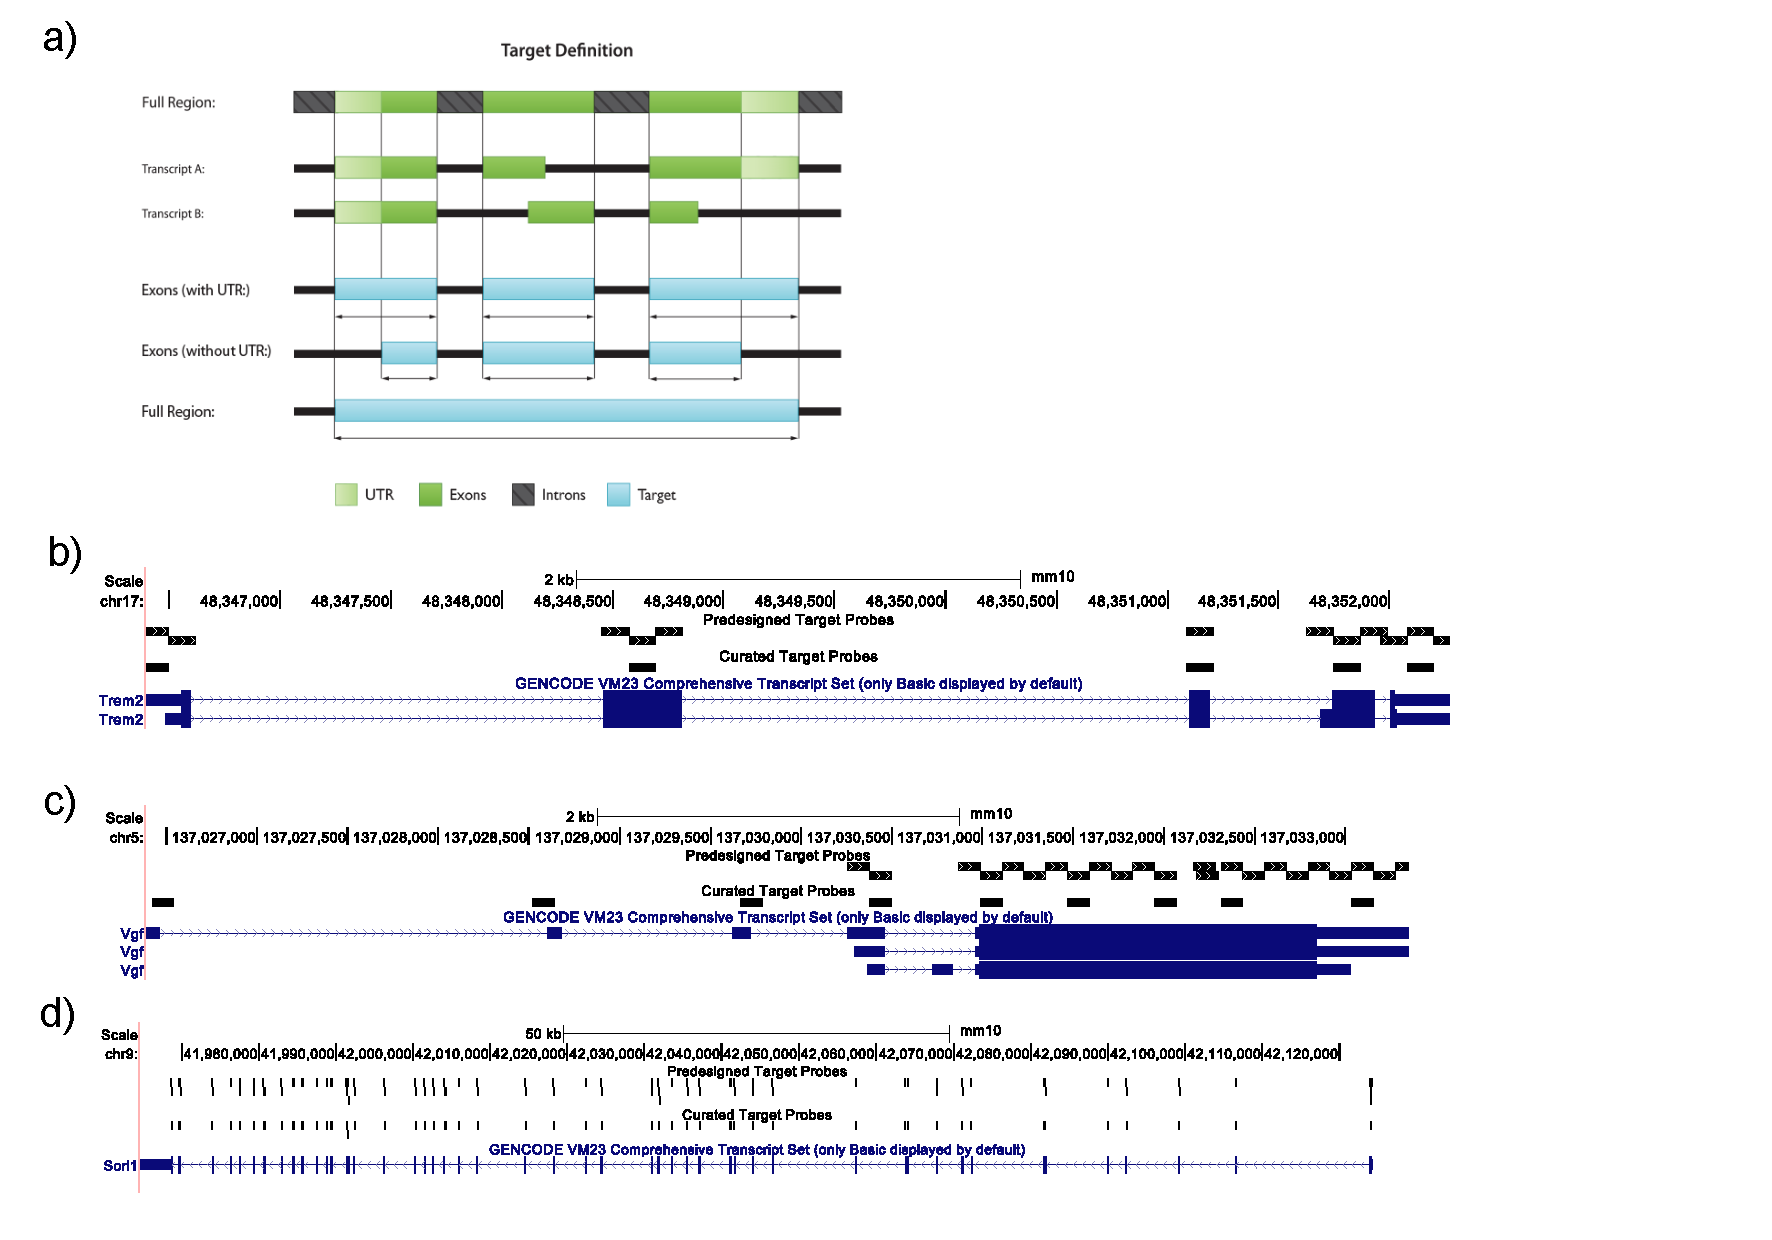
\includegraphics[page=1,trim={0cm 2cm 0cm 0cm},clip,scale = 0.70]{TargetProbes_Visualisation.pdf}
		\end{center}
		\captionsetup{width=1.5\textwidth}
		\caption[Manual curation of probes designed to 20 AD-associated target genes]%
		{\textbf{Manual curation of probes designed to 20 AD-associated target genes.} \textbf{a)} Pre-designed set of probes were provided to "Exons (without UTR)" of target genes. However, exons were unnecessarily covered by contiguous probes which not increases costs but also off-target binding (referred in figure as Predesigned Target Probes). Manual curation was therefore needed for each target gene (referred in figure as Curated Target Probes))to ensure that only exons are covered with one probe for every 500bp. Shown in \textbf{b,c,d)} are UCSC genome browser tracks of predesigned and curated probes to \textit{Trem2}, \textit{Vgf} and \textit{Sorl1} in mouse genome. }
		\label{fig:target_probes_eg}
	\end{figure}
\end{landscape}

\subsubsection{SMRT Bell Template Preparation}
\label{section:ch2_smrtbelltemplate_explanation} 
After pooling the two fractions at equimolar quantities with the SMRTbell Template Prep Kit v1.0 (PacBio), SMRT bell template preparation was performed (\cref{fig:isoseq_labworkflow}, Step 1, 2). This involved repairing DNA damage and polishing ends of fragments for ligation of blunt hairpin adapters, essential to generate high quality library of closed, continous and circular SMRTBell templates. Any abasic sites were filled-in, thymine dimers resolved, and deaminated cytosine are alkylated. 3’ overhangs were removed, whereas 5’ overhangs were filled-in by T4 DNA Polymerase and phosphorylated by T4 PNK. Following 1x AMPure purification of repaired dsDNA, hairpin adapters were then ligated to the blunt ends for up to 24hours (\cref{fig:isoseq_labworkflow}, Step 3). Any fragments failed to ligate were removed with exonuclease III and VII (\cref{fig:isoseq_labworkflow}, Step 4). The repaired, ligated SMRT bell library was then purified twice with 1x AMPure beads, and assessed with Qubit DNA High sensitivity assay (Invitrogen) and Bioanalyzer 2100 (Analyzer) before proceeding to primer annealing and polymerase binding (\cref{fig:isoseq_labworkflow}, Step 5,6). 

\subsubsection{Primer Annealing and Polymerase Binding} 
\label{section:ch2_polbinding_loading}
Post ligation of hairpin adapters, sequencing primer and polymerase were bound to both ends of the SMRTbell templates. The primer and polymerase to template ratio was critical to minimise under- or –over loading, and is dependent on the loading method (Diffusion or MagBead), and concentration and mean library size. The SMRTbell molarity was determined using the previous \textbf{Equation \ref{eqn:isoseq_library_molarity}}.

Prior to the release of v3.0 chemistry in 2018, MagBead Loading was only recommended for IsoSeq SMRTbell libraries, whereas Diffusion Loading was recommended for all other applications with insert sizes from 250bp – 100kb. As suggested by the name, Diffusion loading involves immobilization of polymerase-bound SMRTbells to ZMW by diffusion, whereas Magbead loading involves immobilization by attachment to paramagnetic beads. Magbead loading therefore requires an additional step of hybridising SMRTbell templates to magbeads and washing of SMRTbell-bound Magbeads before loading on the instrument, whereby a built-in Magbead station facilitates movement of Magbeads across ZMW. Typically, Diffusion loading preferentially loads shorter transcripts, whereas magbead loading preferentially loads longer >1b as it rolls across nanowells. However, with the newer release of kits and chemistry, diffusion loading was recommended for all applications including Iso-Seq. Subsequently, all of the samples bar the first two were sequenced by Diffusion Loading. 


\subsubsection{Sequencing} 
\label{section:ch2_sequencing}
Sequencing was performed on the PacBio Sequel 1M SMRT cell. Samples were processed using either the version 3 chemistry (diffusion loading at 5pM, pre-extension 4 hours, Capture time 20 hours) or version 2.1 chemistry (magbead loading at 50pM with a 2 hour pre-extension and 10 hour capture).

Of note, DNA Interal Control Complex (PacBio) was also added to each library before sequencing. Composed of a 1966bp-insert that has already been ligated with SMRTbell adapters and bound by polymerase, this control sequence provides a quality-control measure of loading and sequencing performance. The amount of internal control was similarly determined by the library size and concentration, with PacBio recommending an average number of 500-1000 sequenced reads per SMRT cel.     

\begin{figure}[!htp]
	\begin{center}
		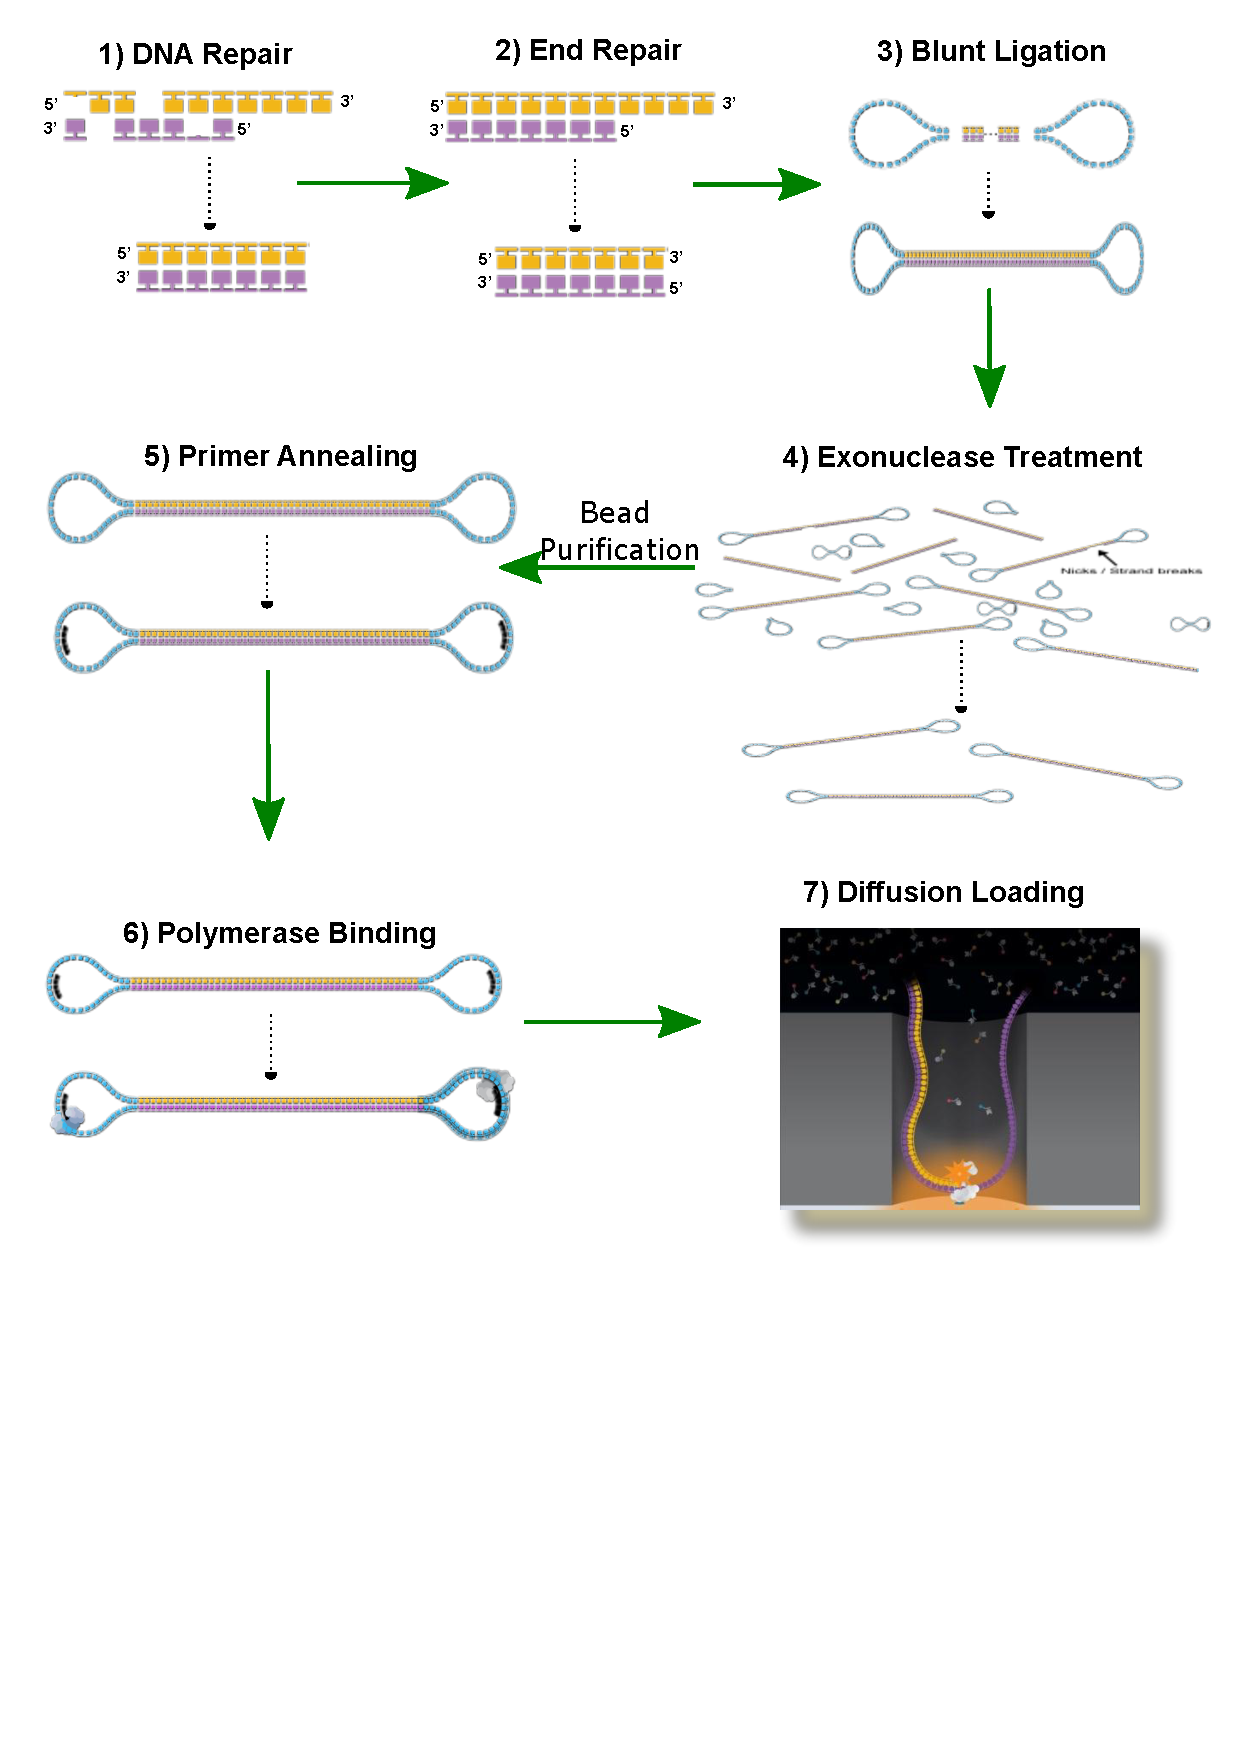
\includegraphics[page=1,trim={0cm 8cm 0cm 0cm},clip,scale = 0.70]{labwork_isoseq.pdf}
	\end{center}
	\captionsetup{width=0.95\textwidth,singlelinecheck=off}
	\caption[Lab workflow of Iso-Seq SMRT Bell Template Preparation, Primer Annealing \& Polymerase Binding]%
	{\textbf{Lab workflow of Iso-Seq SMRT Bell Template Preparation, Primer Annealing \& Polymerase Binding.} Shown is a flow diagram of the lab workflow of Iso-Seq library preparation for long-read sequencing on the Sequel:
	\begin{enumerate}
		\item Repair DNA Damages by repairing abasic sites and nicks, removing thymine dimers, oxidisising guanines, deaminating cytosine; essential to ensure continuous sequence for uninterrupted polymerase processivity 
		\item Repair ends for blunt ligation with removal of 3' hangs and addition of 5' hangs by T4 DNA polymerase; essential for blunt ligation of SMRT bell adapters 
		\item Blunt Ligation by adding hairpin SMRT bell adapters to repaired ends
		\item Exouclease treatment to remove incomplete SMRTbells with Exonuclease III and IV; essential to ensure sequencing of good library 
		\item Annealing of primer to both ends of the SMRT bell templates to initiate sequencing 
		\item Binding of polymerase to both ends of SMRT bell templates for efficieny loading into ZMWs
		\item Immbolisation of polymerase-bound SMRTbels to ZMW by diffusion
	\\
	\end{enumerate} 
	Individual figures and legend are taken and adapted from "PacBio Sequel Library and Sequencing Preparation" presentation
}
	\label{fig:isoseq_labworkflow}
\end{figure}
